\documentclass[../main.tex]{subfiles}
\begin{document}
Create an applet using Java, which takes a number as input and displays its
multiplication table. Use appropriate GUI components and layout in your applet.

\subsection{Code}
\inputminted[frame=lines, breaklines, breakanywhere, numberblanklines=false]{java}{./programs/prog14/Tables.java}

\subsection{Output}
\begin{figure}[h!]
	\centering
	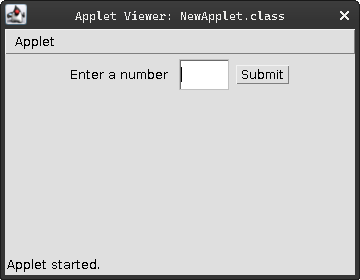
\includegraphics[width=0.3\textwidth]{./assets/p14-s1.png}
	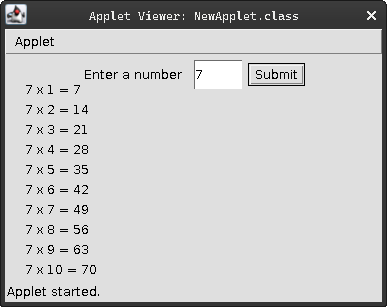
\includegraphics[width=0.3\textwidth]{./assets/p14-s2.png}
\end{figure}
\end{document}
